\documentclass[a4paper,11pt]{article}
\usepackage{amsmath,amsthm,amsfonts,amssymb,amscd,amstext,vmargin,graphics,graphicx,tabularx,multicol} \usepackage[french]{babel}
\usepackage[utf8]{inputenc}  
\usepackage[T1]{fontenc} 
\usepackage[T1]{fontenc}
\usepackage{amsmath,amssymb}
\usepackage{pstricks-add,tikz,tkz-tab,variations}
\usepackage[autolanguage,np]{numprint} 
\usepackage{color}
\usepackage{ulem}

\setmarginsrb{1.5cm}{0.5cm}{1cm}{0.5cm}{0cm}{0cm}{0cm}{0cm} %Gauche, haut, droite, haut
\newcounter{numexo}
\newcommand{\exo}[1]{\stepcounter{numexo}\noindent{\bf Exercice~\thenumexo} : \marginpar{\hfill /#1}}
\reversemarginpar


\newcounter{enumtabi}
\newcounter{enumtaba}
\newcommand{\q}{\stepcounter{enumtabi} \theenumtabi)  }
\newcommand{\qa}{\stepcounter{enumtaba} (\alph{enumtaba}) }
\newcommand{\initq}{\setcounter{enumtabi}{0}}
\newcommand{\initqa}{\setcounter{enumtaba}{0}}

\newcommand{\be}{\begin{enumerate}}
\newcommand{\ee}{\end{enumerate}}
\newcommand{\bi}{\begin{itemize}}
\newcommand{\ei}{\end{itemize}}
\newcommand{\bp}{\begin{pspicture*}}
\newcommand{\ep}{\end{pspicture*}}
\newcommand{\bt}{\begin{tabular}}
\newcommand{\et}{\end{tabular}}
\renewcommand{\tabularxcolumn}[1]{>{\centering}m{#1}} %(colonne m{} centrée, au lieu de p par défault) 
\newcommand{\tnl}{\tabularnewline}

\newcommand{\trait}{\noindent \rule{\linewidth}{0.2mm}}
\newcommand{\hs}[1]{\hspace{#1}}
\newcommand{\vs}[1]{\vspace{#1}}

\newcommand{\N}{\mathbb{N}}
\newcommand{\Z}{\mathbb{Z}}
\newcommand{\R}{\mathbb{R}}
\newcommand{\C}{\mathbb{C}}
\newcommand{\Dcal}{\mathcal{D}}
\newcommand{\Ccal}{\mathcal{C}}
\newcommand{\mc}{\mathcal}

\newcommand{\vect}[1]{\overrightarrow{#1}}
\newcommand{\ds}{\displaystyle}
\newcommand{\eq}{\quad \Leftrightarrow \quad}
\newcommand{\vecti}{\vec{\imath}}
\newcommand{\vectj}{\vec{\jmath}}
\newcommand{\Oij}{(O;\vec{\imath}, \vec{\jmath})}
\newcommand{\OIJ}{(O;I,J)}

\newcommand{\bmul}[1]{\begin{multicols}{#1}}
\newcommand{\emul}{\end{multicols}}


\newcommand{\reponse}[1][1]{%
\multido{}{#1}{\makebox[\linewidth]{\rule[0pt]{0pt}{20pt}\dotfill}
}}

\newcommand{\titre}[5] 
% #1: titre #2: haut gauche #3: bas gauche #4: haut droite #5: bas droite
{
\noindent #2 \hfill #4 \\
#3 \hfill #5

\vspace{-1.6cm}

\begin{center}\rule{6cm}{0.5mm}\end{center}
\vspace{0.2cm}
\begin{center}{\large{\textbf{#1}}}\end{center}
\begin{center}\rule{6cm}{0.5mm}\end{center}
}



\begin{document}
\pagestyle{empty}
\titre{Contrôle 1 : Transformations, aires et fractions }{Nom}{Prénom}{Date}{Classe}

\begin{flushleft}
\begin{tabular}{|m{9.5cm}|m{1.25cm}|m{1.25cm}|m{1.25cm}|m{1.25cm}|m{1.25cm}|}
\hline 
\textbf{Compétences} & \begin{center}
\textbf{N.E.}
\end{center} & \begin{center}
\textbf{M.I.}
\end{center} & \begin{center}
\textbf{M.F.}
\end{center}  & \begin{center}
\textbf{M.S.}
\end{center} & \begin{center}
\textbf{T.B.M.}
\end{center} \\ 
\hline 
Extraire d'un document les informations utiles, les reformuler, les organiser, les confronter à ses connaissances &  &  & & &\\
\hline 
Décomposer un problème en sous-problèmes &  &  & & &\\
\hline



\end{tabular} 
\end{flushleft}

\textit{N.E = Non évalué ; M.I. = Maîtrise insuffisante ; M.F. = Maîtrise fragile ; M.S. = Maîtrise satisfaisante ; T.B.M. = Très bonne maîtrise}\\

\vspace*{0.3cm}




\exo{4} \textit{(Cours)}\\

\q Écrire la formule pour calculer l'aire d'un parallélogramme et d'un disque.\\

\q Calculer l'aire d'un disque de rayon 30 cm.\\


\exo{3} \textit{(Les fractions)}\\
Compléter \textbf{sur le sujet} la pyramide en écrivant dans chaque case la somme des deux cases qui se trouvent en dessous d'elle.\\

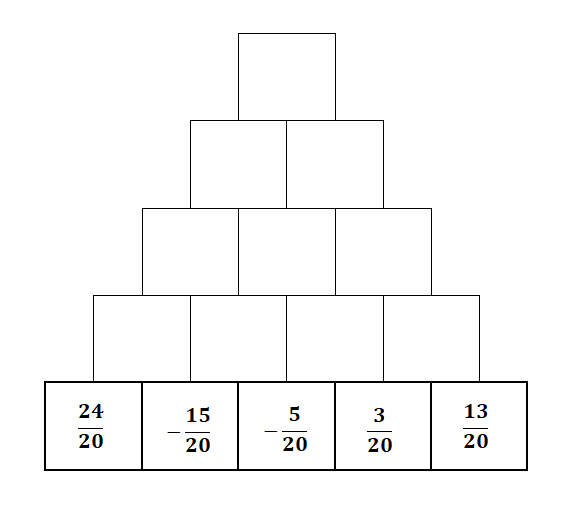
\includegraphics[scale=0.95]{pyramide2.eps} 

\exo{5} \textit{(Les aires)}\\

M. Dupuy habite Malakoff et souhaite vendre son terrain représenté ci-dessous. \\
A Malakoff, le prix d'un mètre carré vaut 5 000 euros.

\bmul{2}

\includegraphics[scale=0.5]{airesmalakoff.eps} 

\columnbreak
\vspace*{1cm}
$\rightarrow$ \textbf{Quel est le prix de ce terrain ?} \textit{Justifier votre réponse par des calculs.}

\emul

\newpage

\vspace*{0.5cm}

\exo{4} \textit{(Les fractions)}\\

Antoine refait la tapisserie de son salon. \\
Il pose $\dfrac{4}{15}$ du papier peint le premier jour, $\dfrac{1}{5}$ le deuxième jour et $\dfrac{2}{6}$ le troisième jour.\\

A-t-il fini de poser tout le papier peint du salon ? \\
\textit{Justifier votre réponse par des calculs.}\\

\vspace*{0.5cm}


\exo{4} \textit{(Les transformations)}\\

\bmul{2}
\initq
\q On considère l'hexagone ABCDEF de centre O représenté ci-contre.\\

\qa Quelle est l'image du quadrilatère CDEO par la symétrie de centre O?\\

\qa Quelle est l'image du segment [AO] par la symétrie d'axe (CF)?\\

\qa On considère la rotation de centre O qui transforme le triangle OAB en le triangle OCD.\\
Quelle est l'image du triangle BOC par cette rotation ?\\


\columnbreak

\includegraphics[scale=0.8]{hexagone1.eps} 

\emul
\vspace*{0.25cm}


\bmul{2}
\q La figure ci-contre représente un pavage dont le motif
de base a la même forme que l'hexagone ci-dessus. On
a numéroté certains de ces hexagones.\\

$\rightarrow$ \textbf{Quelle est l'image de l'hexagone 14 par la translation qui transforme l'hexagone 2 en l'hexagone
12 ?}\\

\columnbreak

\includegraphics[scale=0.75]{nidabeille.eps} 


\emul



\end{document}
